\documentclass[UTF8,fontset=fandol,11pt,a4paper]{ctexart}
\usepackage[margin=23mm,headheight=14pt]{geometry}
\usepackage{amsmath,amssymb,booktabs,tabularx,graphicx}
\usepackage[table]{xcolor}
\usepackage{pgfplots}
\pgfplotsset{compat=1.18}
\usepackage[colorlinks=true,linkcolor=black,urlcolor=blue!45!black]{hyperref}
\usepackage{fancyhdr}
\definecolor{accent}{HTML}{17698B}
\definecolor{faint}{HTML}{EDF3F7}
\definecolor{cA}{HTML}{2679A3}
\definecolor{cB}{HTML}{D67D38}
\definecolor{cC}{HTML}{2D997E}
\definecolor{cD}{HTML}{965FC1}
\pagestyle{fancy}
\fancyhf{}
\fancyhead[L]{\footnotesize Hyser / Hard HiWA 实验}
\fancyhead[R]{\footnotesize 2026-11-17}
\fancyfoot[C]{\footnotesize \thepage}
\setlength{\parindent}{2em}
\setlength{\parskip}{4pt}
\newcommand{\cloud}[1]{%
\begin{tikzpicture}
\begin{axis}[width=\linewidth,height=60mm,view={42}{24},grid=major,grid style={black!7},xlabel={$z_1$},ylabel={$z_2$},zlabel={$z_3$},
tick label style={font=\tiny},scatter,scatter src=explicit symbolic,scatter/classes={
0={mark=*,cA},1={mark=*,cB},2={mark=*,cC},3={mark=*,cD}},
only marks,mark size=.7pt]
\addplot3 table[col sep=comma,x=x,y=y,z=z,meta=cluster]{#1};
\end{axis}
\end{tikzpicture}}
\begin{document}
\begin{center}
{\Huge\bfseries Hyser 数据上的 Hard HiWA}\\[5pt]
{\Large\color{accent} 高密度肌电—手指力量跨模态对齐实验}\\[9pt]
{\large 全部 250 个同步时间窗 · PCA 后标准化与白化核验}\\[6pt]
{\small 实验日期 2026-11-17 \quad 数据来源 PhysioNet Hyser 2.0.0}
\end{center}
\noindent\colorbox{faint}{\parbox{\dimexpr\textwidth-2\fboxsep}{\small
\textbf{结果概述：}PCA 后已经分别实行 Z-score 与协方差白化，并按用户指定的 GCOT/HiWA 算法结构核对重跑。正确计算的配对 $R^2$ 仍低于零；原作者式旋转停止条件被触发，但局部 ADMM 共识残差不小。}}

\section{数据、特征与实验问题}
研究目标是在无配对监督下，以层级最优传输和正交旋转 $R\in O(3)$，将前臂肌电域 $X$ 与实际手指力量域 $Y$ 对齐。数据为 Hyser \texttt{random\_dataset/subject01\_session1/sample1} 的一段 25 秒真实同步记录。
\begin{center}
\rowcolors{2}{faint}{white}
\begin{tabularx}{\textwidth}{>{\bfseries}l X X}
\toprule
 & 肌电域（$X$） & 力量域（$Y$）\\
\midrule
原始观测 & 256 通道、2048 Hz、51,200 采样点 & 5 通道、100 Hz、2500 采样点\\
同步窗口 & 0.1 秒，每通道去均值 RMS & 0.1 秒，逐指窗口均值\\
降维与选择 & 通道 Z-score 后 PCA 到 3 维 & 选拇指、中指、食指 3 维\\
点云规模 & $250\times3$ & $250\times3$\\
\bottomrule
\end{tabularx}
\end{center}
肌电特征处理为 $\operatorname{PCA}_3(\operatorname{Zscore}_{256}(\log(1+10^5\mathrm{RMS})))$，前三主成分解释方差为 $86.32\%$、$5.01\%$ 和 $2.22\%$，合计 \textbf{$93.55\%$}。

\section{PCA 降维后进行统一度量}
本次专门检查两种后处理：
\begin{align}
\text{逐维 Z-score:}\quad &\widetilde x_{ij}=\frac{x_{ij}-\bar x_j}{s_j},\\
\text{协方差白化:}\quad &\widetilde X=(X-\bar X)\Sigma_X^{-1/2},\quad
\widetilde Y=(Y-\bar Y)\Sigma_Y^{-1/2}.
\end{align}
白化后的两域协方差均近似 $I_3$，与 HiWA 的 \texttt{normal()} 操作一致。PCA 肌电主成分相互正交，因此肌电侧 Z-score 与白化近似等价；力量侧仍存在跨坐标相关性，二者不等价。

\noindent\textbf{诊断：}利用同步配对直接求最优正交 Procrustes，Z-score 后最高 $R^2=-0.1892$，白化后最高 $R^2=-0.1369$。这个上界只针对当前三维表示和零时延同步定义，不等于 HiWA 性能。

\clearpage
\section{最初的真实硬聚类散点图}
\begin{center}
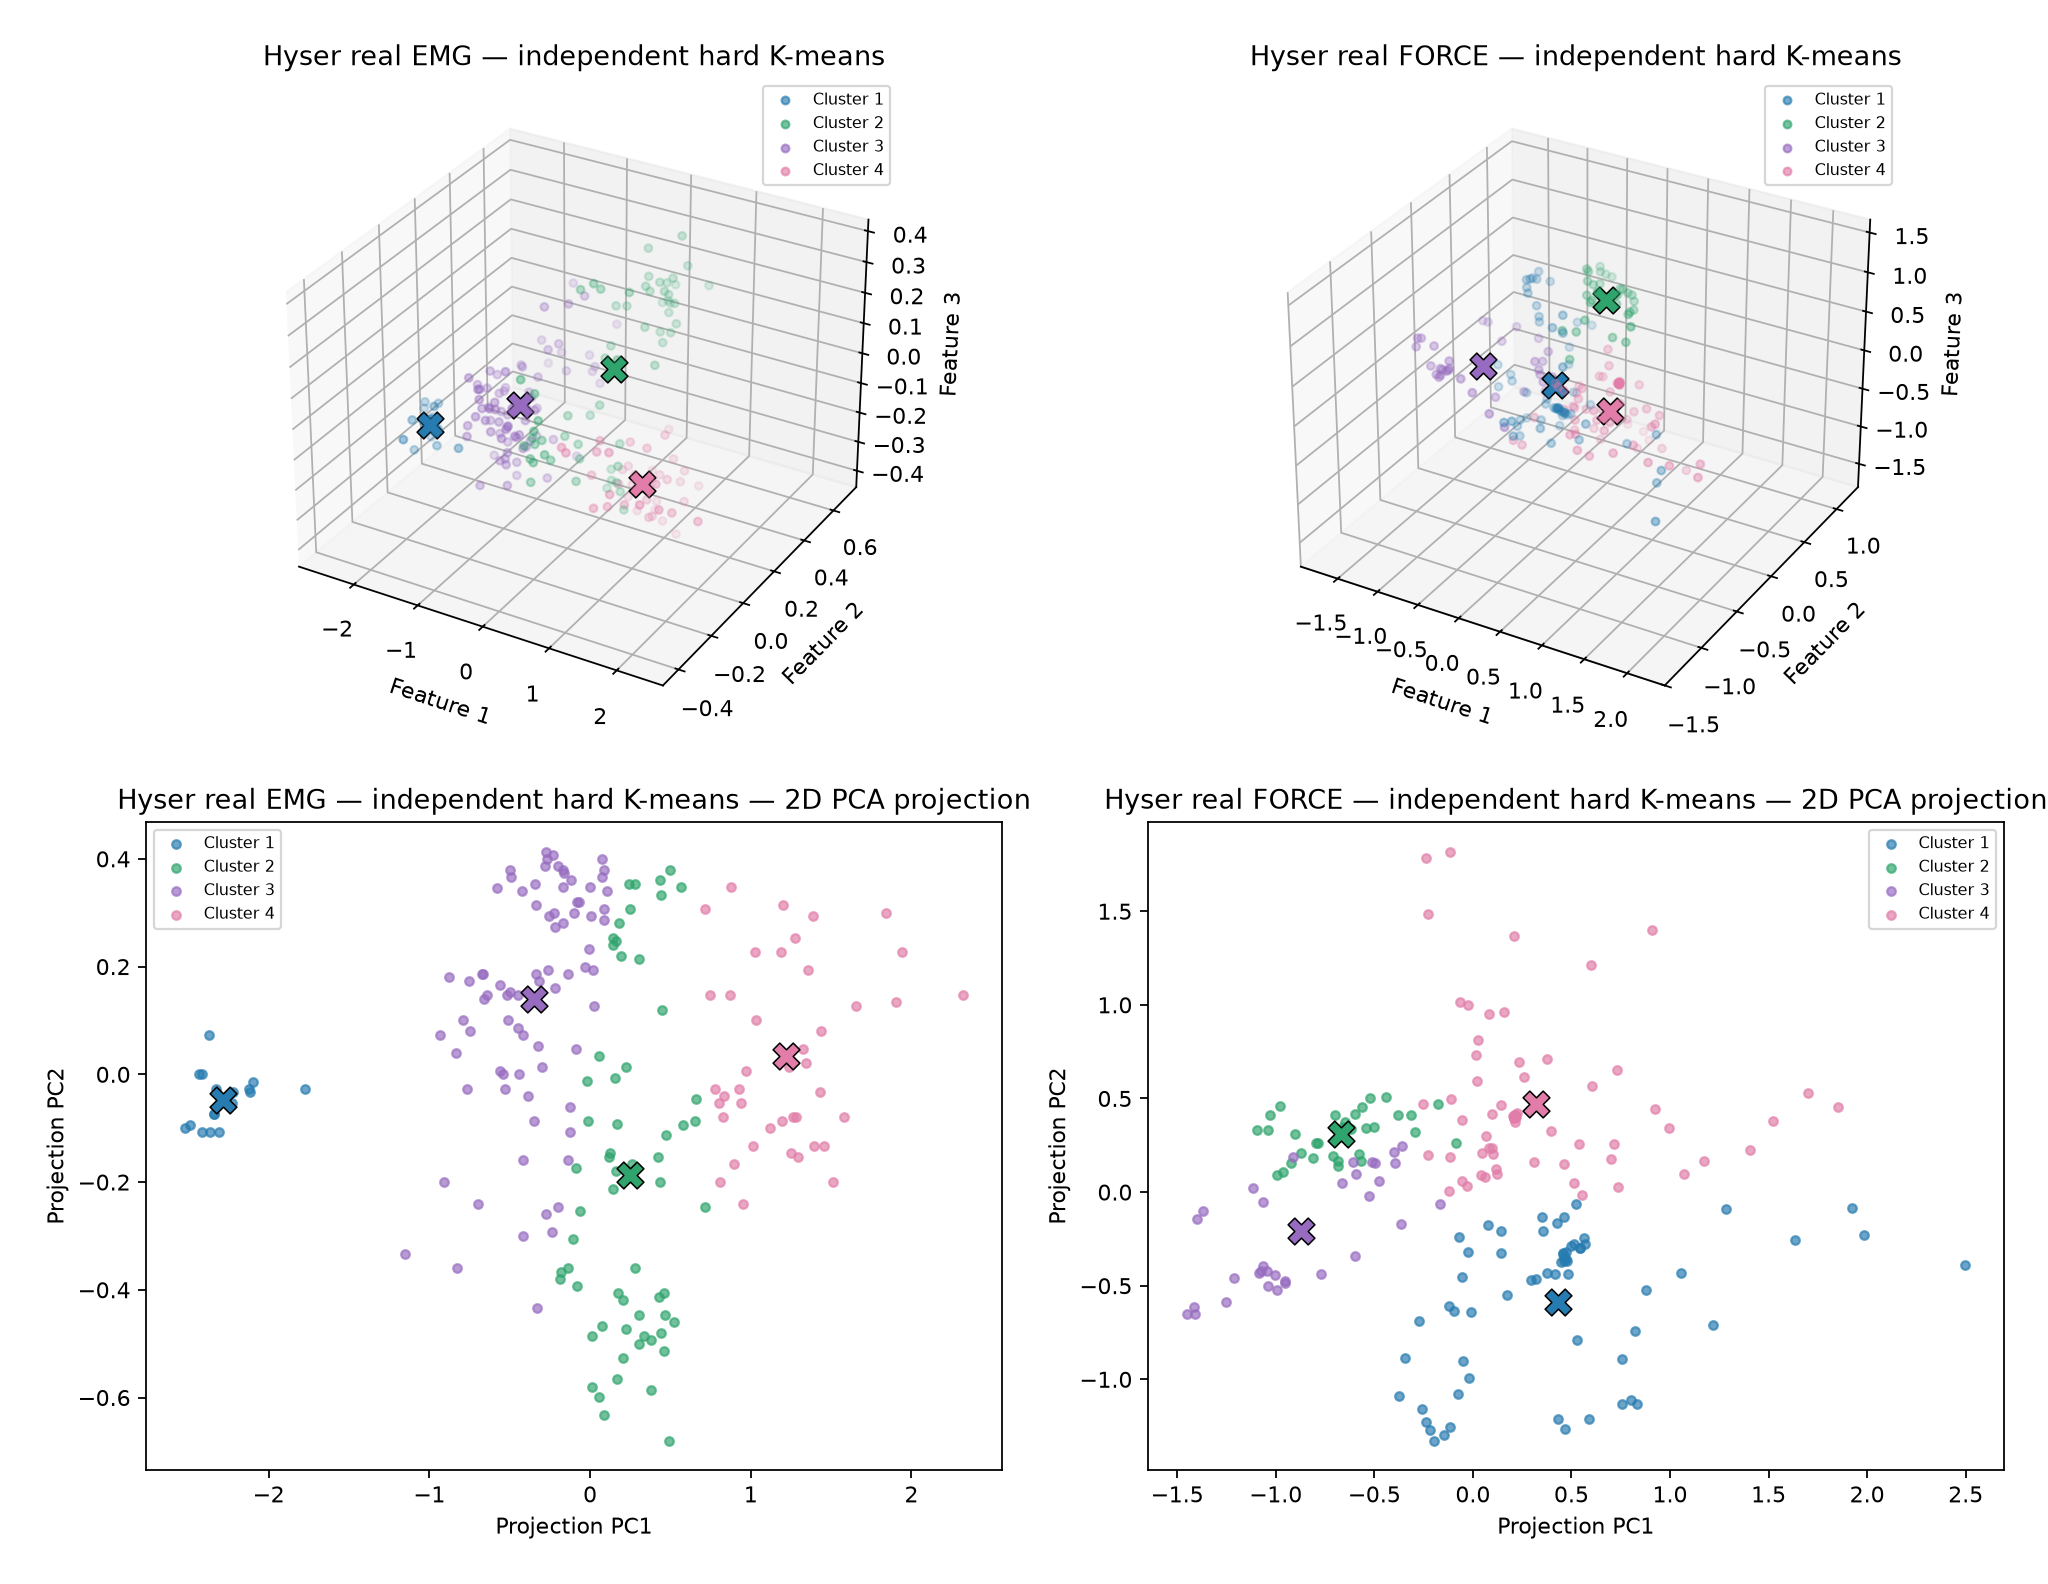
\includegraphics[width=\textwidth,height=0.69\textheight,keepaspectratio]{figures/initial200_hard_clusters_fourpanel.png}
\end{center}
\noindent\small
图1：依照用户指定的原始四联图样式，由此前已保存的真实 Hyser \textbf{200 个窗口}的独立 K-means 簇坐标重新生成。上排为两域3D簇，下排为2D PCA投影。源域和目标域的簇标签各自独立，颜色相同并不表示已经匹配。
\normalsize

\clearpage
\section{全量250点白化后的硬分组与对齐散点图}
\begin{center}
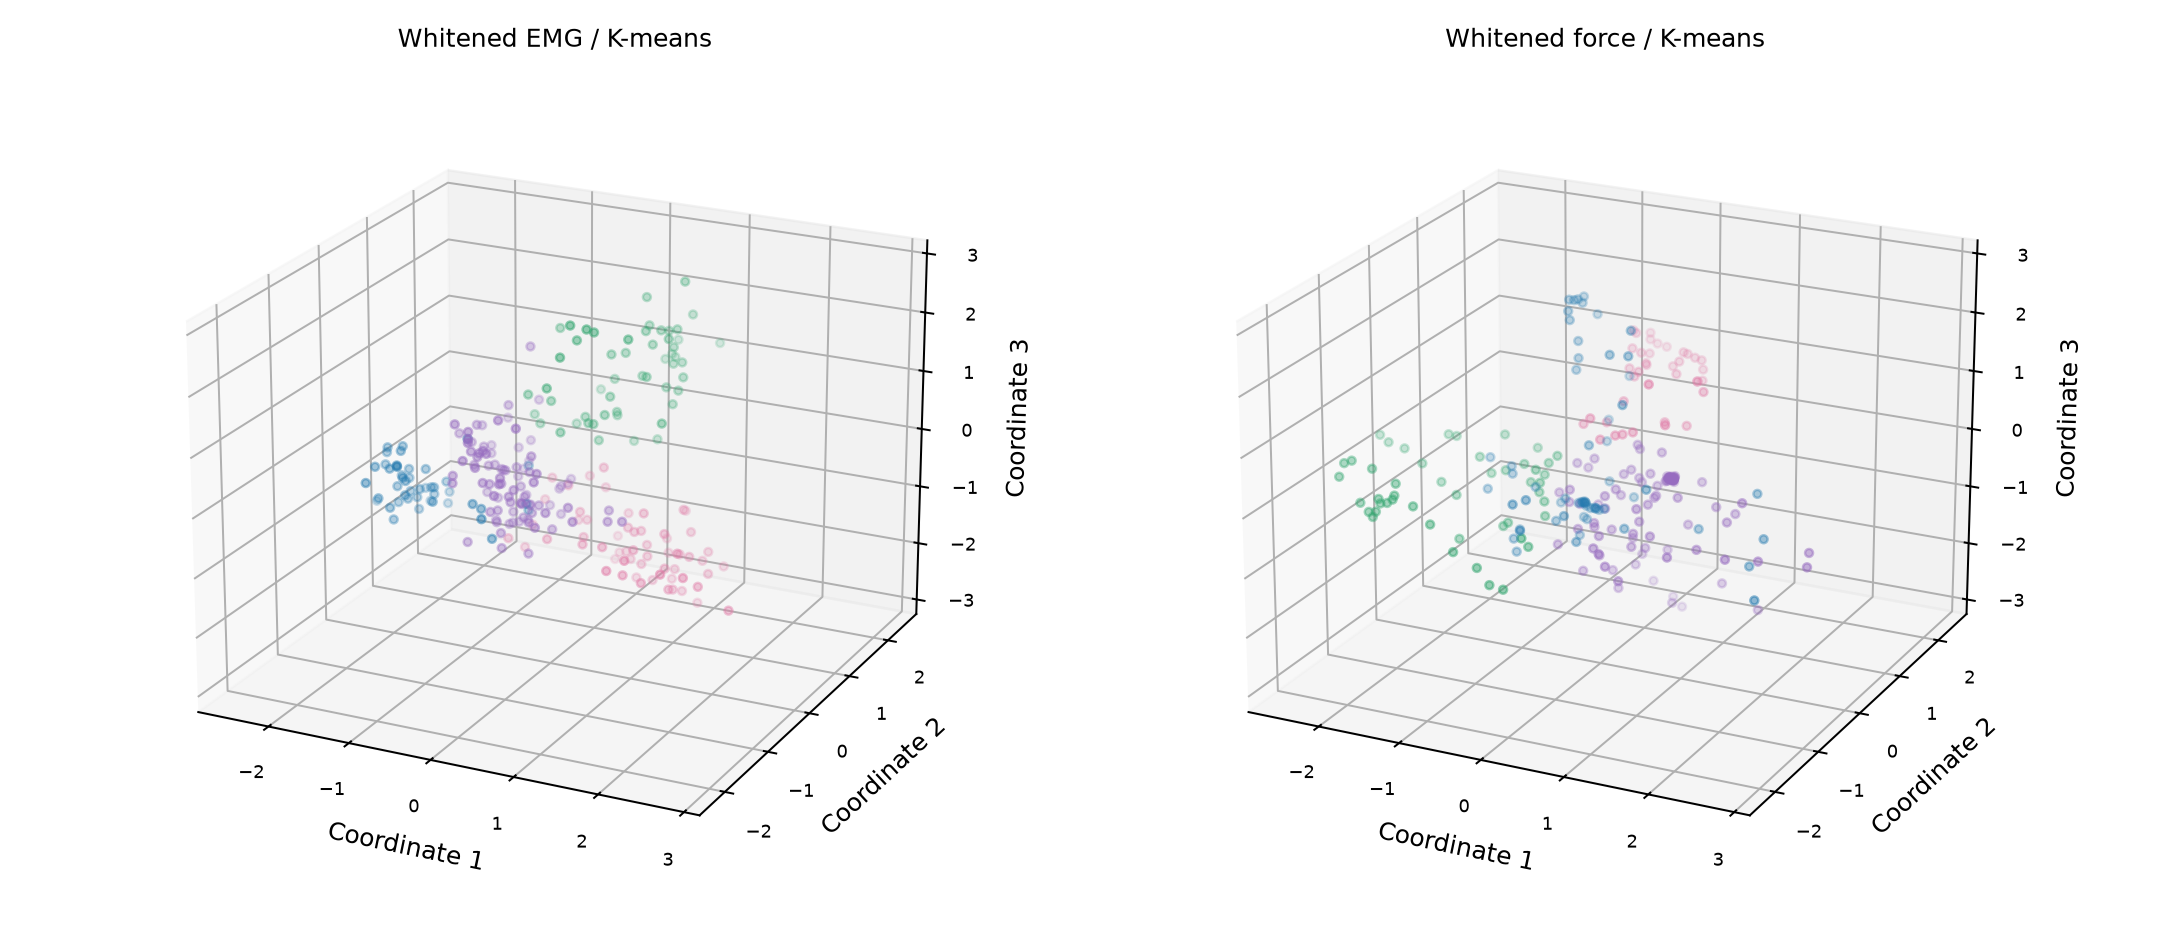
\includegraphics[width=\textwidth,height=0.29\textheight,keepaspectratio]{figures/all250_whitened_hard_clusters_3D.png}
\end{center}
\noindent\small
图2：全部250点经过HiWA协方差白化后，两域独立K-means硬分组。与图1的初始200点特征尺度不同，不应直接比较原坐标范围。
\normalsize

\begin{center}
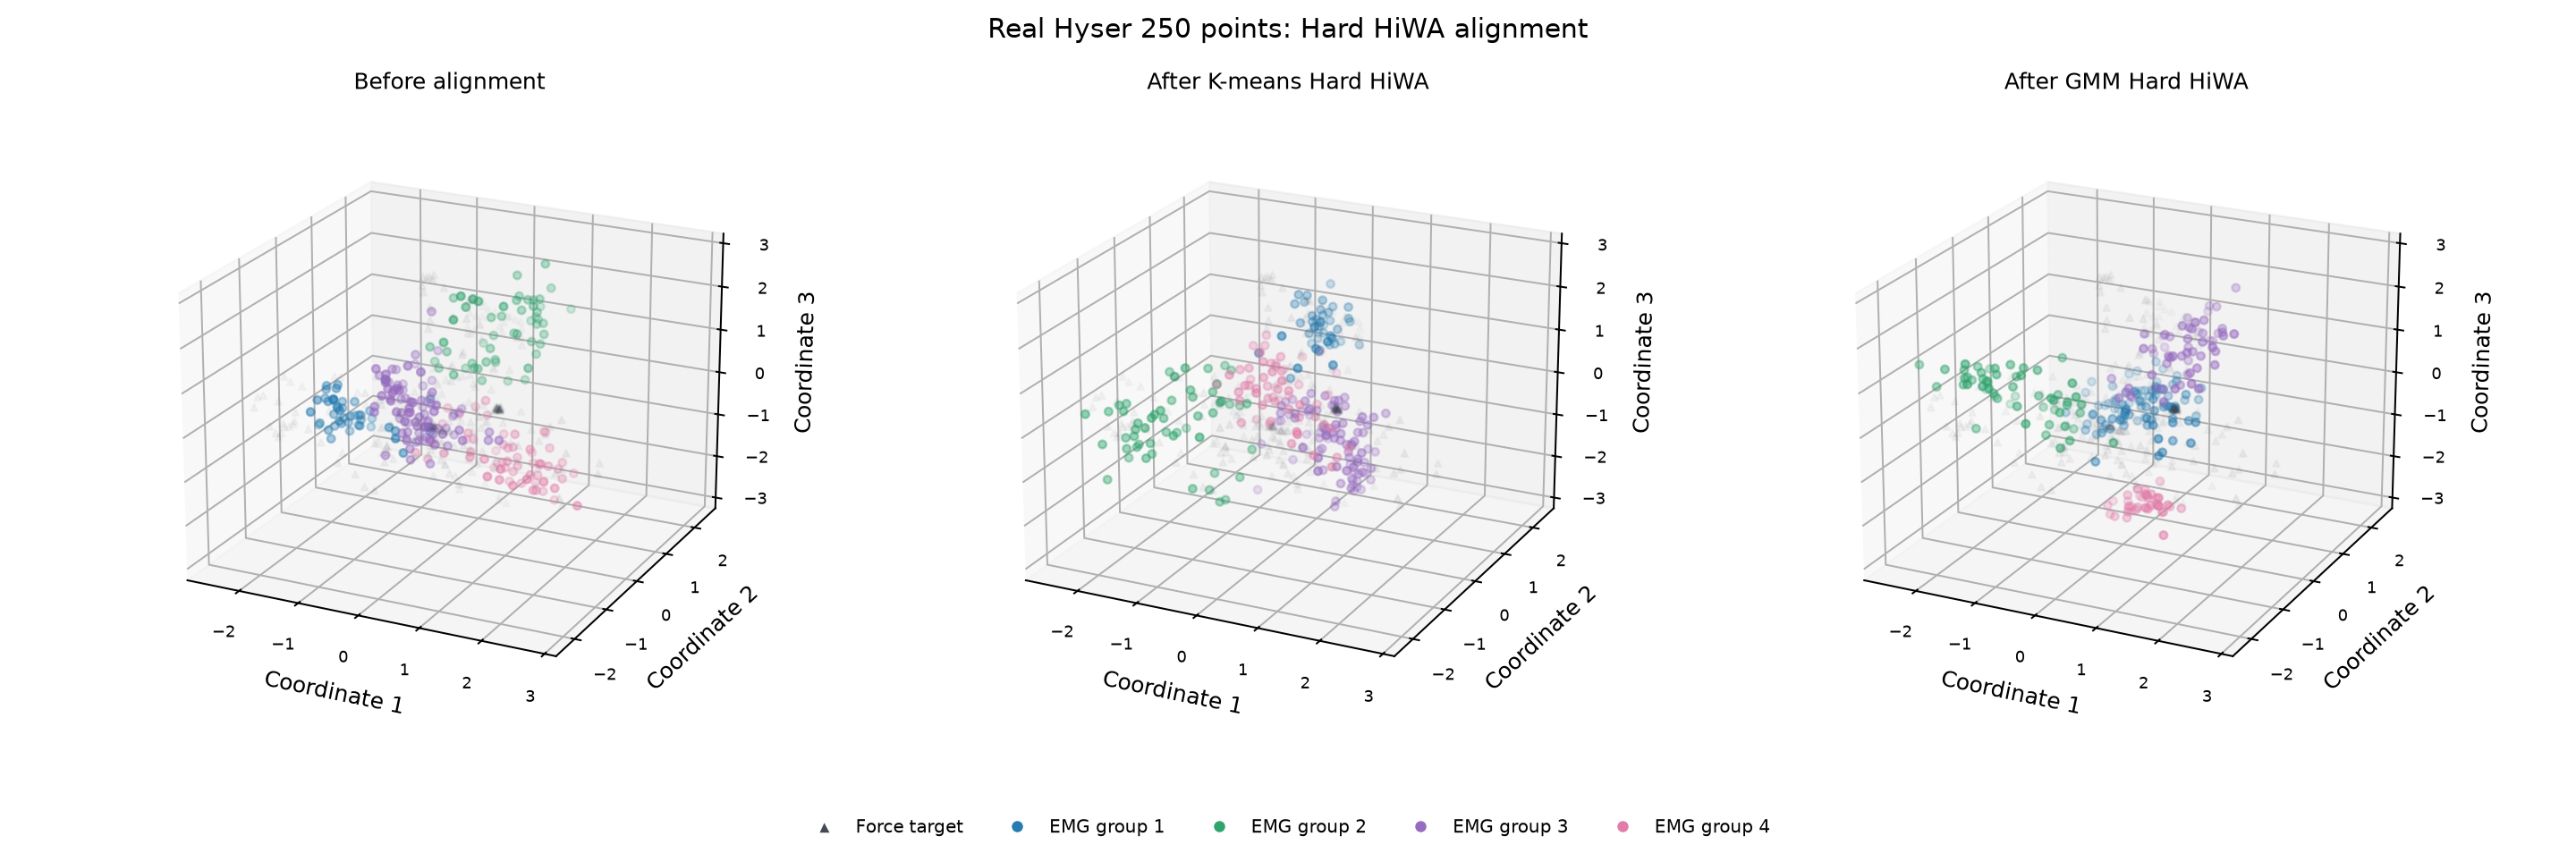
\includegraphics[width=\textwidth,height=0.30\textheight,keepaspectratio]{figures/all250_after_hard_hiwa_3D_overlay.png}
\end{center}
\noindent\small
图3：Hard HiWA对齐前与对齐后的三维点云叠加。灰色三角形为目标力量域，彩色圆点为源肌电域的四个硬簇。三个视图使用相同坐标范围；中间为K-means/3D HiWA，右侧为GMM/Isomap HiWA。图中旋转来自已保存的真实数据数值运行结果，而非合成示意。
\normalsize

\clearpage
\section{Hard HiWA对齐后的二维散点图}
\begin{center}
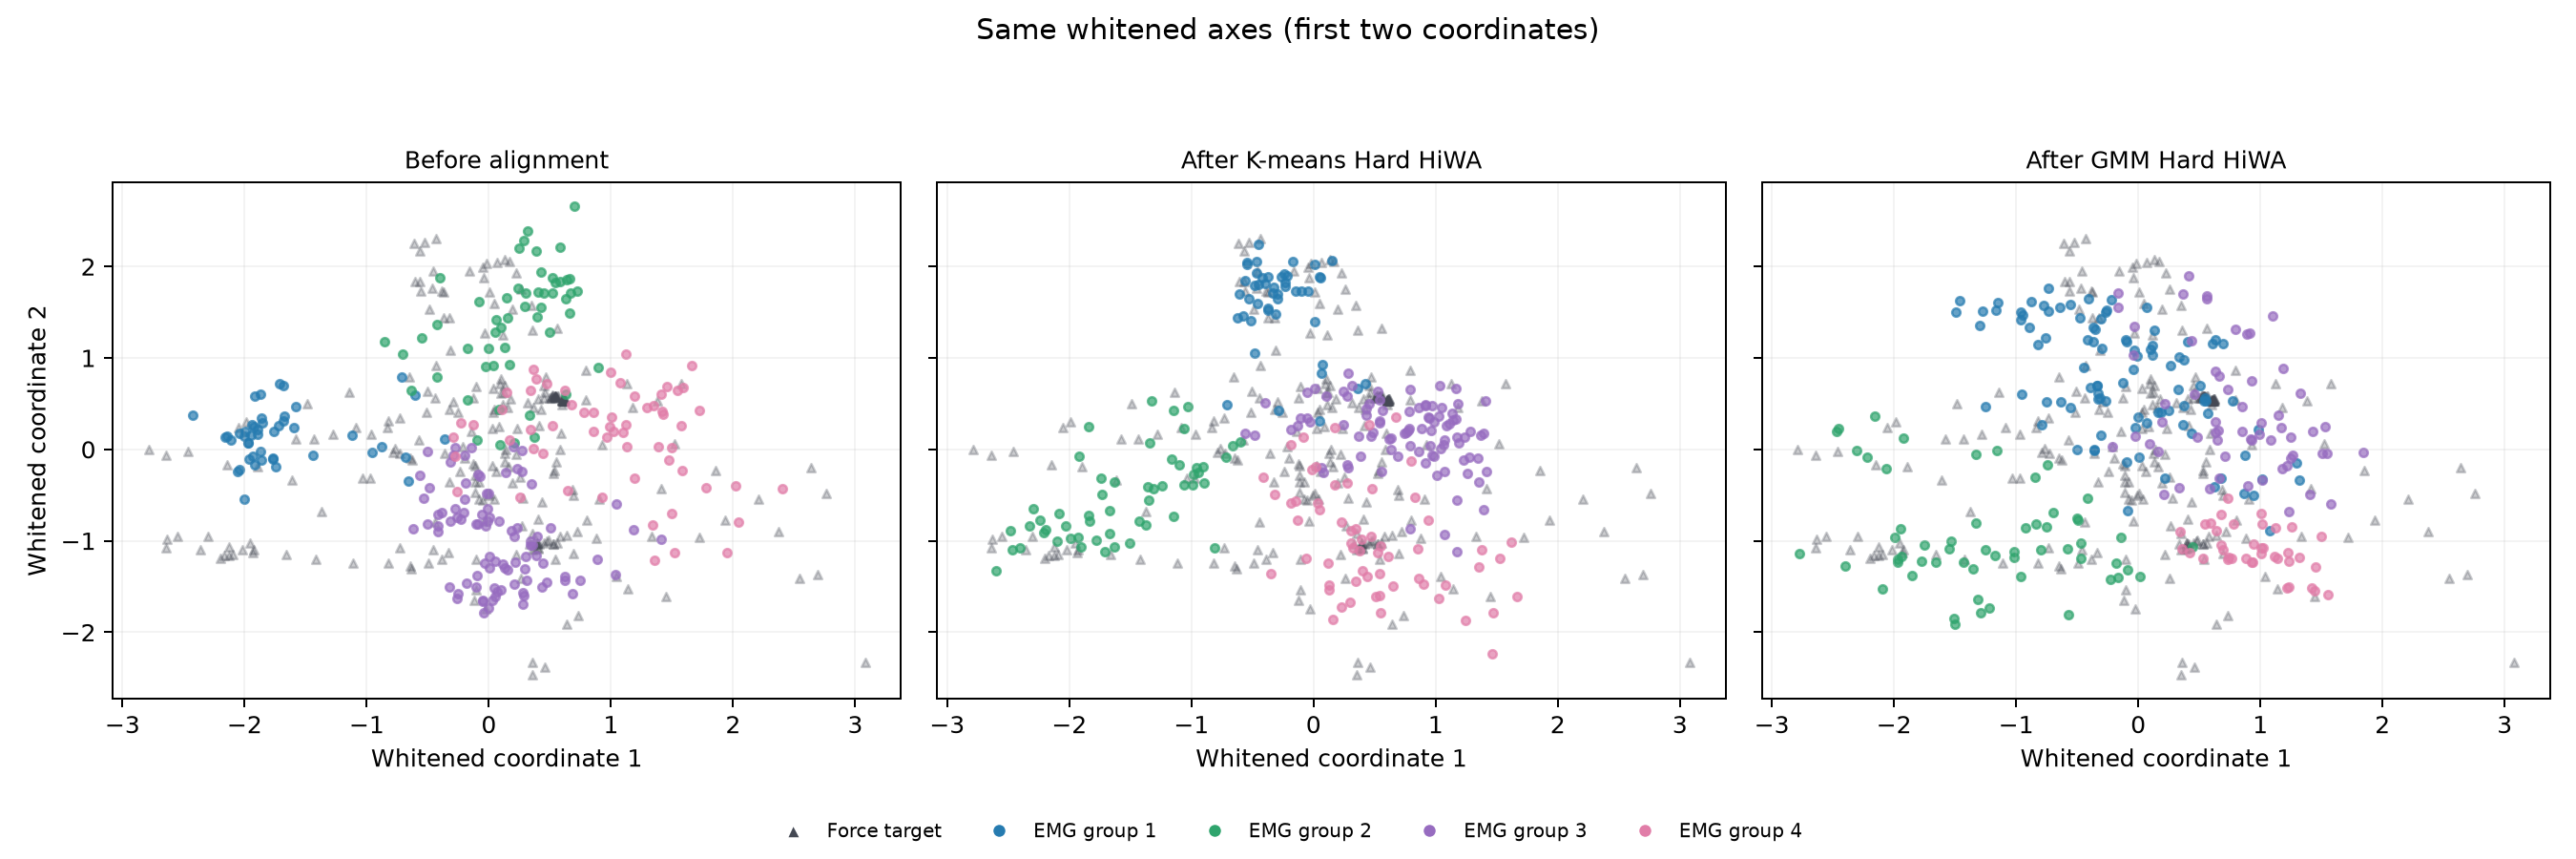
\includegraphics[width=\textwidth,height=0.40\textheight,keepaspectratio]{figures/all250_after_hard_hiwa_2D_overlay.png}
\end{center}
\noindent\small
图4：共同白化三维坐标的第1、2维投影；没有重新做二维PCA。采用同轴范围与图例以直接比较对齐前后的源域—目标域重叠。
\normalsize

\clearpage
\section{HiWA 设定、指标与实测结果}
使用用户提供的 \texttt{GCOT-reproducible-20261018} 包中 \texttt{gcot/alignment.py} 的层级 OT / Procrustes / ADMM 更新形式，并按其 HiWA 作者默认参数：
\begin{center}
\rowcolors{2}{faint}{white}
\begin{tabular}{ll@{\qquad}ll}
\toprule
参数 & 取值 & 参数 & 取值\\
\midrule
组数 $K$ & 4 & 随机种子 & 42\\
$\mu$ & 0.005 & 外层最大迭代 & 300\\
簇级熵 $\varepsilon_g$ & 0.2 & 簇级 Sinkhorn 次数 & 1000\\
样本熵 $\varepsilon_s$ & 0.1 & 样本 Sinkhorn 次数 & 150\\
局部最大迭代 & 100 & 局部旋转阈值 & 0.01\\
全局旋转阈值 & 0.1 & 停止方式 & legacy\\
\bottomrule
\end{tabular}
\end{center}
样本真实同步对应 $\pi(i)$ \textbf{不参与模型求解}，只用于事后计算：
\begin{align}
R^2 &=1-\frac{\sum_i\|R x_i-y_{\pi(i)}\|^2}{\sum_i\|y_{\pi(i)}-\bar y\|^2},\\
\mathrm{rMSE}_{\mathrm{paired}}&=
\frac{\sum_i\|R x_i-y_{\pi(i)}\|^2}{\sum_i\|y_{\pi(i)}\|^2}.
\end{align}
后者为新代码评估文件的\emph{配对数据相对平方误差}，不是需要真实 $R_{\mathrm{gt}}$ 的旋转 rMSE。白化及 Z-score 的全量目标都已中心化，故本次 $R^2=1-\mathrm{rMSE}_{\mathrm{paired}}$。

\begin{center}\small
\rowcolors{2}{faint}{white}
\begin{tabular}{llrrr}
\toprule
归一化 & 方法 & $R^2\uparrow$ & rMSE$\downarrow$ & 平均距离$\downarrow$\\
\midrule
白化 & 对齐前 & -0.6741 & 1.6741 & 1.9775\\
白化 & K-means / 3D & -0.8876 & 1.8876 & 2.2116\\
白化 & GMM / Isomap & -1.1681 & 2.1681 & 2.3979\\
Z-score & 对齐前 & -0.7096 & 1.7096 & 2.0019\\
Z-score & K-means / 3D & -1.2254 & 2.2254 & 2.3650\\
Z-score & GMM / Isomap & -1.2939 & 2.2939 & 2.4509\\
\bottomrule
\end{tabular}
\end{center}
\noindent\textbf{收敛诊断：}白化 + K-means 在第 88 次外层迭代满足全局变化条件（$\Delta R=0.0893$），但局部共识残差为 $0.9110$；白化 + GMM / Isomap 在第 43 次停止（$\Delta R=0.0731$），局部残差为 $1.8680$。这些是原作者式停止，不代表 ADMM 严格收敛。

\clearpage
\section{结果分析与实验边界}
\begin{center}
\begin{tikzpicture}
\begin{axis}[width=.92\textwidth,height=7cm,ybar,bar width=13pt,
symbolic x coords={白化KMeans,白化GMM,ZscoreKMeans,ZscoreGMM},
xtick=data,x tick label style={rotate=15,anchor=east,font=\small},
ylabel={$R^2$（越大越好）},ymin=-1.5,ymax=.25,
ymajorgrids,grid style={black!10},enlarge x limits=.12,
nodes near coords,every node near coord/.append style={font=\scriptsize}]
\addplot[fill=accent!70] coordinates {
(白化KMeans,-0.8876) (白化GMM,-1.1681)
(ZscoreKMeans,-1.2254) (ZscoreGMM,-1.2939)};
\end{axis}
\end{tikzpicture}
\end{center}
\noindent\textbf{结论：}PCA 后统一尺度确实已完成核验，两域白化后协方差均接近 $I_3$。但是在当前三维特征和零时延同步定义下，Hard HiWA 依然未降低配对误差。对全部白化点做有监督的最优正交 Procrustes，其最高 $R^2$ 仍仅为 $-0.13693$，说明不能只靠修改 HiWA 实现或标准化顺序消除几何不相容。

\noindent\textbf{复现状态：}本次实测结果由针对指定 GitHub 分支源码逐项核对的\emph{本地公式移植版本}得到，并非在本地容器直接导入该远程分支的原始 Python 文件。源码核对及参数见仓库的 \texttt{experiments/hyser/} 实验笔记。该试验全部 250 点用于无监督拟合与评价，不能提供跨试次泛化结论。

\par\noindent\small
数据：\href{https://physionet.org/content/hd-semg/2.0.0/}{PhysioNet Hyser 2.0.0}；实验项目：
\href{https://github.com/noelabernathy400-bot/ot-hiwa}{ot-hiwa GitHub 仓库}。
\end{document}
